\chapter{Fundamentals}
\label{cha:fundamentals}
This chapter covers fundamentals that are necessary for a better understanding of the concepts presented in this work. It gives a short introduction into mobile communications systems which our system uses. Mobile communications systems are used in our system to estimate the users coarse location. Furthermore, state of the art analytical mobility models for mobile network simulations are presented. Another section covers the data (provided by A1) our system is using to generate driving trajectories. At last, the process to estimate the coverage area for cell sites with Voronoi tessellation is shown.
\section{Global System for Mobile Communications}
%\section{GSM}
Mobile communication networks are the basis of our modern communication and interaction. However the beginning of wireless communication began in the late \nth{19} century and was shaped by the work of Hughes, Maxwell, Hertz, Tesla and Faraday.

In 1982, a new mobile communication network was developed by the Group Spécial Mobile (GSM) of the CEPT (Conférence Européenne des Administrations des Postes et des Télécommunications). The main goal of GSM was to develop a Europe-wide standard for digital mobile communication. Over the past two centuries, there has been a rapid increase in the use of GSM all over the world. The present section is based on the books \emph{GSM: Switching, Services and Protocols} by Jörg Eberspächer et al.\ \cite{Eberspaecher2001} and \emph{Mobilfunknetze und ihre Protokolle 1} by Bernhard Walke \cite{Walke2001}.

Besides GSM, there are other mobile communication currently in use. These systems are known as 3G (UMTS, HSPA, WCDMA, etc.\ ) and 4G (LET, LTE Advanced, etc.\ ) networks whereas GSM is a network of the second generation (2G).

\subsection{Components - System architecture}
GSM consists of a large number of components which are necessary for its operation. However, we will only focus on components that are necessary to understand the functionality of our system. The overview of a GSM network with GPRS capability is visible in Figure~\ref{fig:GSMNetwork}.  The various standardized interfaces which are responsible for communication between the components can be seen as well as the different components of the \emph{Radio Access Network} RAN and the \emph{Core Network} CN. The RAN consists of a BTS and BSC in GSM and a Node B and a RNC in GPRS.
\begin{figure}
	\centering
	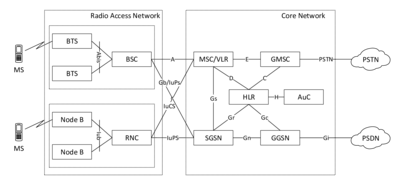
\includegraphics[width=\linewidth]{./images/GSMNetwork}
	\caption{System overview of the a GPRS Network}
	\label{fig:GSMNetwork}
\end{figure}

\subsubsection{Mobile Station}
Mobile stations (MS) are the equipment used by mobile subscribers to access services provided by the network operator. The mobile station consist of two components, first the \emph{Mobile Equipment} and second the \emph{Subscriber Identity Module} (SIM). The SIM grants a mobile subscriber access to the network and allows to initiate or receive calls.
For management purposes GSM assigns the following numbers and identities to a MS:
\begin{itemize}
	\item \textbf{IMSI} International Mobile Station Identity
	\item \textbf{TMSI} Temporary Mobile Station Identity
	\item \textbf{MSISDN} Mobile Station International ISDN Number
	\item \textbf{MSRN} Mobile Station Roaming Number

\end{itemize}
\subsubsection{Base Transceiver Station}
The base transceiver station (BTS) provides the radio channels for signaling and user traffic data with in a cell. The mobile station establishes a connection with the BTS over the air interface. The BTS consists only of a few parts, the high-frequency equipment (transceiver and receiver) and the signaling and protocol processing unit. The control remains in the BSC.
\subsubsection{Base Station Controller }
A base station controller (BSC) is used to manage one or more BTS. It is directly connected to a MSC. Together with the BTS, the BSC forms the \emph{Base Station Subsystem} (BSS). For example, the BSC executes the handover protocol and switches a MS to a new BTS.
\subsubsection{Mobile Switching Center - MSC}
The mobile switching center (MSC) together with the databases (HLR, VLR) forms the \emph{Mobile Switching System} (MSS). The MSC is responsible for the switching in the network. For example, the MSC performs signal routing, routing path search and service processing. Additionally the MSC has to pay attention to the allocation and administration of radio channel and the mobility of subscribers. A \emph{Public Land Mobile Network} (PLMN) can consists of several MSCs where each is responsible for a dedicated area.
Furthermore, the MSC is connected to a \emph{Gateway Mobile Switching Center} (GMSC) which forwards voice traffic between fixed and mobile networks. The GMSC enables the subscriber to call subscribers in different MSCs or PLMNs.
\subsubsection{Visited Location Register - VLR}
The visited location register (VLR) stores information of all MS who are located in the serving area of the associated MSC. A VLR can be assigned to one or more MSCs. A MS can be registered in a VLR of its home PLMN or a foreign one when a roaming agreement exists.
\subsubsection{Home Location Register - HLR}
Typically, there is one home location register (HLR) per PLMN and one VLR for each MSC. The HLR stores all permanent and temporary subscriber information for all registered subscribers. Moreover, it stores a coarse current location of each MS. The HLR operates as a central register needed by the MSC for routing of subscribers.
\subsection{Radio Resource Management}
The GSM standard~\cite{Etsi1994} distinguishes between two modes of operation first idle and second connected mode. The radio resource management (RRM) is necessary to manage the physical and logical channels.
\paragraph{Idle Mode}
In idle mode there is no dedicated channel assigned to a MS. However, the MS listens on signaling channels (BCCH and CCCH). The higher layers are only informed when a MS reaches the boundaries of a location area.
\paragraph{Connected Mode}
\label{subsub:connected}
In this mode there are two dedicated channels assigned to the MS, the first one is SACCH and the second one is either FACCH or SDCCH.
The radio resource management provides the following service to a connected MS (a full list can be found in ETSI GSM 04.08 \cite{Etsi1994}):
\begin{itemize}
	\item Transfer of messages on any data link layer
	\item Establishment/release of multiframe mode on SDCCH, FACCH or SACCH.
	\item Automatic cell reselection and handover to maintain the RR-connection
\end{itemize}
\subsubsection{Handover}
A handover is the transfer of an established connection to a new BTS. A handover is necessary for various reasons. First of all, a handover decision is made by the GSM network and not by the MS. As mentioned before the handover protocol is implemented in the BSS. The BSS decides to initiate a handover based on BSS criteria (channel quality, received signal level, distance between MS and BTS) and network criteria (e.g.\ traffic load of the network).

Handovers are only performed when the MS is in connected mode. If the MS is in idle mode and reaches the boundaries of the cell a location area update is performed if the new cell is in a different location area.

The GSM standard does not define an algorithm for handover decision. Therefore, network suppliers are responsible for implement them. A basic handover algorithm is specified in appendix A of the ETSI GMS 05.08 \cite{Etsi19942}.
\paragraph{Intra-Cell-Handover} The channel within the cell will be changed, e.g.\ when the channel is noisy. The change can either be done to a new frequency or to a new time-slot with the same (old) frequency.
\paragraph{Inter-Cell/Intra-BSC-Handover}
The channel will be changed between two cells within the same BSC.
\paragraph{Intra-Cell/Intra-MSC-Handover}
The connection will be changed between two cells in different BSCs, but both are managed by the same MSC.
\paragraph{Inter-MSC-Handover}
The connection will be changed between two cells that are managed by different MSCs.
\\

The first two handovers can be carried out by the BSC if it supports the handover protocol. If this is not the case then also Intra-Cell-Handover have to be carried out by the MSC.

\paragraph{Ping-pong Handover}
A ping-pong handover is an undesirable effect where a handover is made to a neighbor cell and after short time back to the original cell \cite{Junius1995}.
\subsubsection{Location Area Updates}
Location area updates (LAU) are used to ease the localization of mobile subscribers. Therefore, a MS must initiate a location area update once it leaves the location area. The HLR and VLR both store the current location area. A MS constantly measures the received signal strengths of all surrounding BTSs and reports it to the BSS to the one with the highest signal strength. If it connects to a BTS outside of the current location area then the MS initiates a location area update and tells the CN its new location area.
There are two cases which can distinguished:
\begin{itemize}
	\item change within the same VLR
	\item change to a new VLR
\end{itemize}

\subsubsection{Location Area}
A location area (LA) defines the area within the mobile network in which the mobile subscriber is located. Location areas are used to decrease the signaling necessary to locate a mobile subscriber within the network. Without location areas, the PLMN has to initiate a paging request to all BTSs. By using location areas, only the BTS within the location area have to carry out the paging request.

%\begin{figure}
%\centering
%\def\svgwidth{200pt}
%\input{images/locationarea.pdf_tex}
%\caption{Example for three location areas}
%\label{fig:locationarea}
%\end{figure}
\begin{figure}
	\centering
	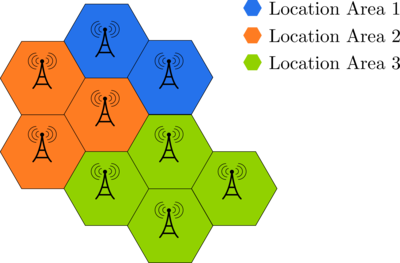
\includegraphics[width=0.7\linewidth]{./images/locationarea}
	\caption{Example for three location areas}
	\label{fig:locationarea}
\end{figure}

One or more BTS with the same MSC can be part of one location area, in most cases they are part of the same BSC. Figure~\ref{fig:locationarea} shows that a location area can consists of several BTS. Each location area is uniquely defined by the \emph{Location Area Identity} (LAI). The LAI (see Tab.\ \ref{tab:lai}) consists of the Mobile Country Code (e.g.\ Austria 232) which identifies the country, the Mobile Network Code (e.g.\ A1 1) which identifies the PLMN and the Location Area which identifies the location area within the PLMN. Together with the Cell-ID (CID) the LAI forms the Global Cell-ID (GCID).
The size of a location area depends on:
\begin{itemize}
	\item Cell density
	\item Voice and data traffic
	\item Network operator configuration
\end{itemize}

\begin{table}
	\begin{tabular}{|c|c|c|}
		\hline  \multicolumn{3}{ |c| }{Location Area Identity} \\
		\hline Mobile Country Code & Mobile Network Code & Location Area Code \\
		\hline 3 digits            & 2 or 3 digits       & 5 digits           \\
		\hline
	\end{tabular}
	\caption{Parts of the Location Area Identity }
	\label{tab:lai}
\end{table}

\subsubsection{Updates}
For its operation the MSC (HLR, VLR) needs to know where the mobile subscriber is located. Therefore, location area updates are required. There are two kinds of location area updates first normal updates and second periodic updates. Normal location area updates (NLAU) happen either when the MS is switched on or off during an IMSI attach/detach or when a MS connects to a new BTS in a different location area. Periodic location area updates (PLAU) are defined by the network operator. Each MS has a PLAU timer for this purpose, whenever the timer expires the MS performs a PLAU.
\subsection{Antennas}
Antennas enable wireless communication between a receiver and a transmitter. In GSM, they are the direct air interface between the MS and the Radio Access Network (RAN). Antennas can be designed to transmit or receive signals equally in all directions (omni-directional antennas) or transmit and receive signals in a specific direction (directional or high gain antennas). In GSM networks, a combination of both is used. Omni-directional are mainly used in rural areas to cover a large area whereas directional antennas are used to cover a smaller area with a higher traffic load.
\subsubsection{Sector}
Sector antennas are a special use case of directional antennas where several directional antennas are combined and each covering a particular sector such as a $120\,^{\circ}$ horizontal pattern. In GSM the most common installations of sector antennas are $60\,^{\circ}$, $90\,^{\circ}$ and $120\,^{\circ}$. Based on the traffic load, smaller sectors can be used with larger ones on the same tower (e.g.\ two $60\,^{\circ}$ antennas with two $120\,^{\circ}$ antennas).
\subsubsection{Antenna size}
The antenna size or more general its coverage is defined by the antenna gain, the antenna characteristics and the transmit power. In mobile communication networks there are four different types of cells in use that are distinguished by their coverage.
\paragraph{Macrocell} Provides the primary radio coverage for mobile networks. Macrocell antennas are mounted on ground-based towers, buildings or other existing infrastructure in order to have a clear view over the coverage area.
\paragraph{Microcell} A microcell offers additional capacity within the coverage of a macrocell. Typically, microcell antennas are mounted at street level. Microcells have lower output power than macrocell and therefore a decreased coverage (e.g.\ 300 to 1000 meters).
\paragraph{Picocell} To provide coverage inside buildings or to a high numbers of users. The coverage of a picocell is 200 meters or less.
%Picocells provide more localised coverage than microcells, inside buildings where coverage is poor or there are high numbers of users.
\paragraph{Femtocell} A low-powered, coverage is on the order of 10 meters, base station designed for use in a home or small business \cite{Zhang2011}.

\section{Mobility Models}
Mobile networks permit its subscribers to move freely within the coverage area. To evaluate and ensure the mobility, mobile network operators need to understand the user mobility. A user mobility can be described by a mobility model. A mobility model describes the user behavior and activity using simulation and analytic models. Simulation models are based on realistic mobility scenarios whereas simplified assumptions about the users movement behavior are the foundation of analytic models.

Two major analytic models which are used in mobile network simulation are the \emph{Random Walk} \cite{Akyildiz2000,Bettstetter2001,Bettstetter2002} and the \emph{Manhattan Mobility Model} \cite{Markoulidakis1997,Buruhanudeen2007}.



%\subsection{Mobility}
\subsection{Random walk}
The mobility of entities in nature is unpredictable, therefore a variety of models exists in literature. These models try to describe the mobility for different scenarios. The random walk model is a memory-less system and maintains no record of previous locations and speed. In each iteration dices a new direction and speed within a predefined range \cite{Camp2002}. An example for a generated random walk is depicted in Figure~\ref{fig:randomwalk}. The speed is limited to the interval $0..5$ and angle is limited to $-15..15^\circ$.
The mobility of entities in nature is unpredictable, therefore a variety of models exists in literature. These models try to describe the mobility for different scenarios. The random walk model is a memory-less system and maintains no record of previous locations and speed. In each iteration dices a new direction and speed within a predefined range \cite{Camp2002}. An example for a generated random walk is depicted in Figure~\ref{fig:randomwalk}. The speed is limited to the interval $0..5$ and angle is limited to $-15..15^\circ$.
%\begin{figure}
%        \centering
%%        \begin{subfigure}[b]{0.5\textwidth}
%                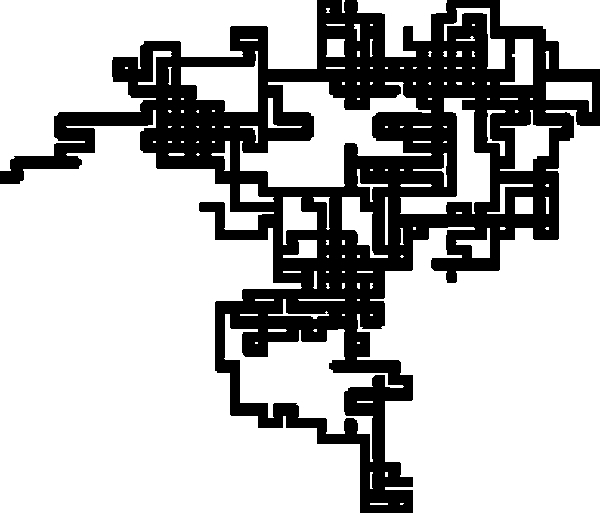
\includegraphics[width=0.7\textwidth]{randomwalksteps1000size3}
%                \caption{Random Walk}
%                \label{fig:randomwalk}
%%        \end{subfigure}%
%%        ~ %add desired spacing between images, e. g. ~, \quad, \qquad etc.
%%          %(or a blank line to force the subfigure onto a new line)
%%        \begin{subfigure}[b]{0.5\textwidth}
%%                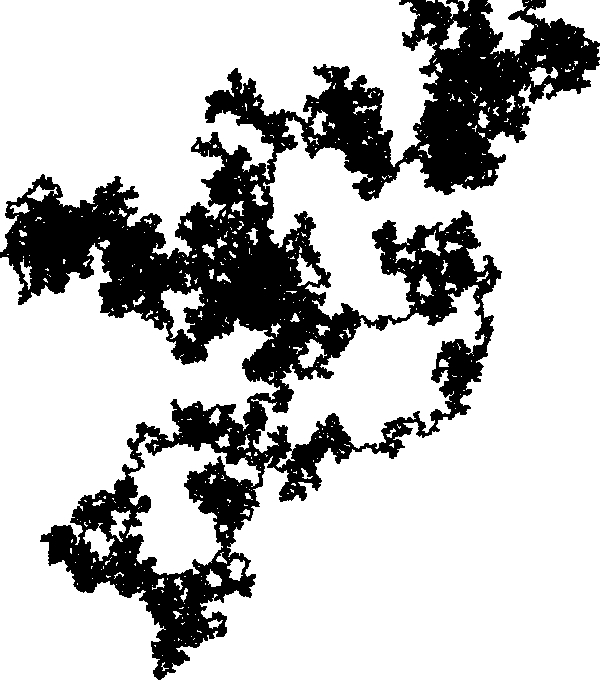
\includegraphics[width=\textwidth]{wiener250000opacity}
%%                \caption{Wiener Process}
%%                \label{fig:distmoc}
%%        \end{subfigure}
%%        \caption{Two random walks with differne(a) and Mobile Originated Calls on Monday, \nth{22} November 2010}\label{fig:random}
%\end{figure}
\begin{figure}
	\centering
	%\tikzsetnextfilename{randomwalk}
	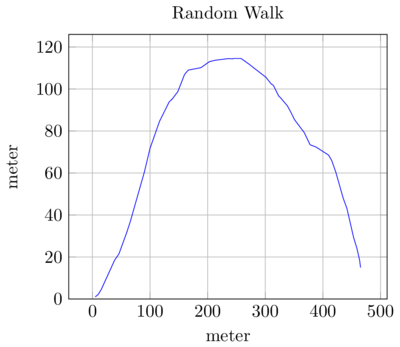
\includegraphics[width=0.7\textwidth]{./images/randomwalk}
	%	\begin{tikzpicture}
	%		\begin{axis}[ymin=0,xmajorgrids,ymajorgrids,xlabel={meter},ylabel={meter},title={Random Walk}]
	%			\addplot table[mark=none]{random.csv};
	%		\end{axis}
	%	\end{tikzpicture}
	\caption{Example for a random walk}
	\label{fig:randomwalk}
\end{figure}

\subsection{Manhattan Mobility Model}
In a Manhattan grid scenario streets are aligned in a square grid. It is named after the district Manhattan in the City of New York. Figure~\ref{fig:manhattan} shows a map of Manhattan and its road network. It can be seen that roads consist of straight lines and each junction forms a right angle.

The Manhattan mobility model can work on any road network~\cite{Zhou2004}. At each junction, the logic is executed which decides if the current street shall be used or a different one. The logic can be modeled as a random number generator with a defined probability density function. For example the probability to drive straight can be $60\%$, turn right $30\%$ and turn left $10\%$. The Manhattan Grid mobility model is an extension to the random walk model where participants are not allowed to move freely, but rather move on a defined road network.
\begin{figure}
	\centering
	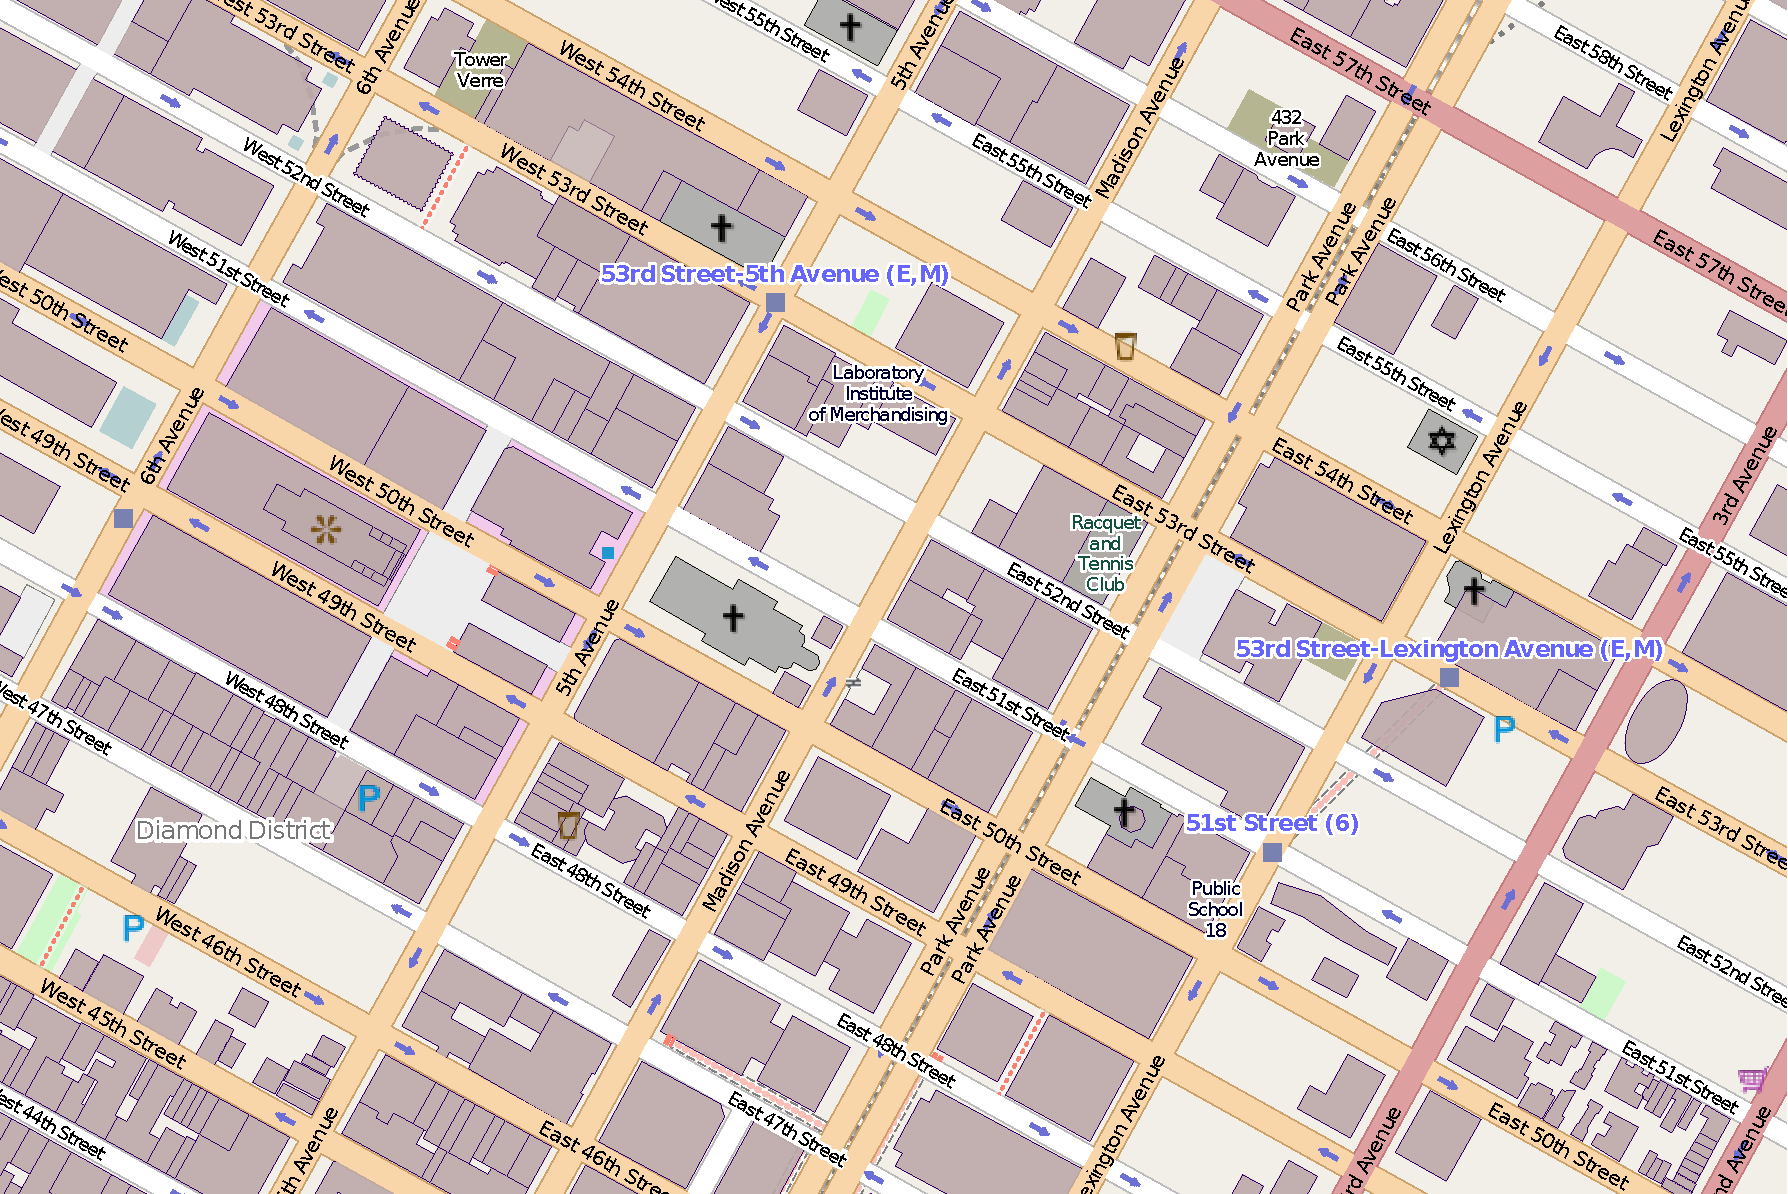
\includegraphics[width=\linewidth]{./images/manhattan}
	\caption{Manhattan Road Network}
	\label{fig:manhattan}
\end{figure}

%\subsection{OD Matrix}
\section{A1 Data}
We are using mobile subscription data from A1. A1 is the largest network operator in Austria with $5.3$ million subscribers. The used data was recorded on the network of A1 between Monday, \nth{22} November 2010 and Sunday, \nth{28} November 2010. The captured interfaces, events and the data structure of the system will be depicted in the succeeding subsections.

Figure~\ref{fig:disthandover} shows the distribution of handover events for Monday, \nth{22} November 2010. It can be seen from this that the distribution for handover events changes over time. A strong increase of handover events takes place at 17 o'clock. This is due to the end of work of subscribers. People are leaving from work and start calling there friends while on their way home.
%On the other hand, a strong decrease of call activity (see Figure~\ref{fig:distmoc}) takes place between 12 and 13 o'clock where people are having lunch.


\begin{figure}
\centering
%\tikzsetnextfilename{hauf_event_32_time_mat}
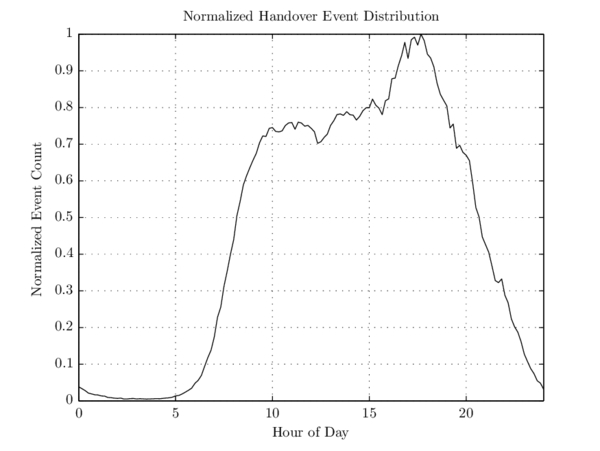
\includegraphics{./images/hauf_event_32_time_mat}
%% This file was created by matlab2tikz v0.4.7 running on MATLAB 8.2.
% Copyright (c) 2008--2014, Nico Schlömer <nico.schloemer@gmail.com>
% All rights reserved.
% Minimal pgfplots version: 1.3
%
% The latest updates can be retrieved from
%   http://www.mathworks.com/matlabcentral/fileexchange/22022-matlab2tikz
% where you can also make suggestions and rate matlab2tikz.
%
\centering
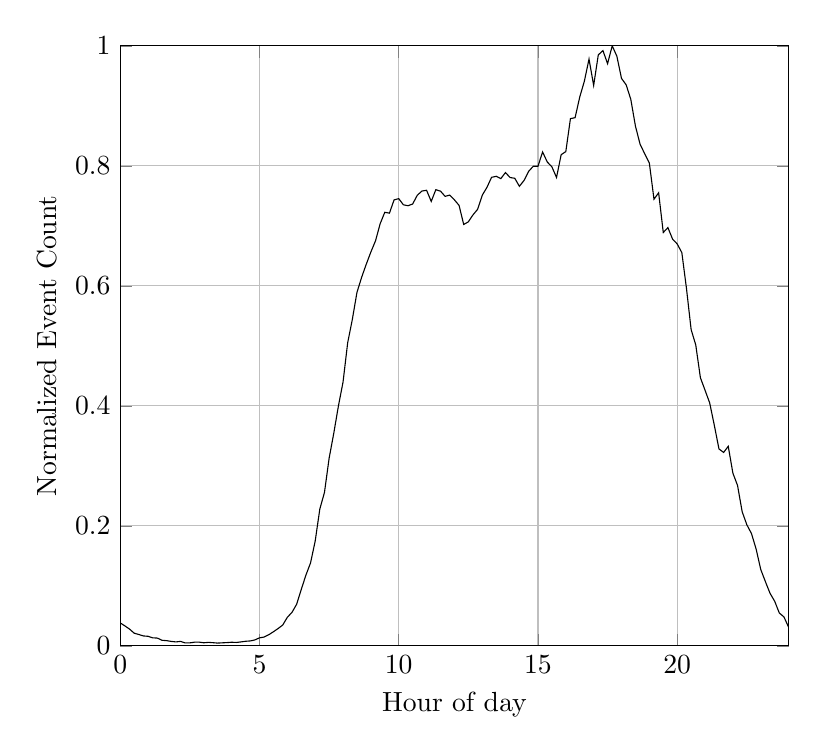
\begin{tikzpicture}

\begin{axis}[%
width=0.7\textwidth,
height=3in,
scale only axis,
xmin=0,
xmax=24,
xlabel={Hour of day},
xmajorgrids,
ymin=0,
ymax=1,
ylabel={Normalized Event Count},
ymajorgrids,
]
\addplot [color=black,solid,forget plot]
  table[row sep=crcr]{0	0.0380908578483074\\
0.166666666666667	0.0332080352171853\\
0.333333333333333	0.0278376219408874\\
0.5	0.0210908889711146\\
0.666666666666667	0.0188292983190226\\
0.833333333333333	0.0164363002590109\\
1	0.0158622573717827\\
1.16666666666667	0.0132998129173482\\
1.33333333333333	0.0128779259761323\\
1.5	0.00924001563056536\\
1.66666666666667	0.00856914623223839\\
1.83333333333333	0.00731731776731898\\
2	0.00647008579520501\\
2.16666666666667	0.00740722809905352\\
2.33333333333333	0.00482403510652645\\
2.5	0.00492777779698939\\
2.66666666666667	0.00604474076430698\\
2.83333333333333	0.00615194154445201\\
3	0.0050661013842733\\
3.16666666666667	0.00575426123101077\\
3.33333333333333	0.00519405070251092\\
3.5	0.00456467838036912\\
3.66666666666667	0.00500039768031344\\
3.83333333333333	0.00539807799375469\\
4	0.00597212088098293\\
4.16666666666667	0.00560902146436266\\
4.33333333333333	0.0064839181539334\\
4.5	0.00757321640379422\\
4.66666666666667	0.00812305266324777\\
4.83333333333333	0.0098175166074757\\
5	0.0132686901102093\\
5.16666666666667	0.0146138869965454\\
5.33333333333333	0.0184834893508128\\
5.5	0.0234527642239874\\
5.66666666666667	0.0287228928995045\\
5.83333333333333	0.034539399744793\\
6	0.0475037779629777\\
6.16666666666667	0.055751321854781\\
6.33333333333333	0.0691652517316384\\
6.5	0.0939217157657767\\
6.66666666666667	0.11779636693098\\
6.83333333333333	0.138181805606947\\
7	0.174515953896748\\
7.16666666666667	0.228019517458166\\
7.33333333333333	0.255618531210988\\
7.5	0.312469525584677\\
7.66666666666667	0.3540150150254\\
7.83333333333333	0.399516559062443\\
8	0.439516282415268\\
8.16666666666667	0.505047081891022\\
8.33333333333333	0.543826099586067\\
8.5	0.589002583192992\\
8.66666666666667	0.613980364966785\\
8.83333333333333	0.635883905013193\\
9	0.65636962828994\\
9.16666666666667	0.67496377651058\\
9.33333333333333	0.703520681105344\\
9.5	0.722543632446564\\
9.66666666666667	0.72111889949754\\
9.83333333333333	0.743181511669324\\
10	0.745290946375403\\
10.1666666666667	0.735027336198937\\
10.3333333333333	0.733457363483265\\
10.5	0.736327577919406\\
10.6666666666667	0.750965671543726\\
10.8333333333333	0.757906057535696\\
11	0.75923050588394\\
11.1666666666667	0.740729726084716\\
11.3333333333333	0.760184938636199\\
11.5	0.757753901589684\\
11.6666666666667	0.749081012666982\\
11.8333333333333	0.751211195911155\\
12	0.743254131552648\\
12.1666666666667	0.734052154908585\\
12.3333333333333	0.702220439384875\\
12.5	0.706598380922411\\
12.6666666666667	0.718189897536803\\
12.8333333333333	0.727516365409421\\
13	0.751010626709593\\
13.1666666666667	0.763905843134136\\
13.3333333333333	0.780788236962137\\
13.5	0.782496533265094\\
13.6666666666667	0.778668427987011\\
13.8333333333333	0.788769507948419\\
14	0.780428595635199\\
14.1666666666667	0.779235554694875\\
14.3333333333333	0.765863121894203\\
14.5	0.775628767156447\\
14.6666666666667	0.790813238950539\\
14.8333333333333	0.799358178555003\\
15	0.799223313057401\\
15.1666666666667	0.823049550967055\\
15.3333333333333	0.806412681506482\\
15.5	0.798303461201963\\
15.6666666666667	0.780553086863755\\
15.8333333333333	0.818571324828738\\
16	0.823633968123329\\
16.1666666666667	0.878700588221055\\
16.3333333333333	0.880191024874039\\
16.5	0.914585184852184\\
16.6666666666667	0.941105274624192\\
16.8333333333333	0.977850935586164\\
17	0.934016190775892\\
17.1666666666667	0.984912354717007\\
17.3333333333333	0.992001438565308\\
17.5	0.970212015478409\\
17.6666666666667	1\\
17.8333333333333	0.982678428782372\\
18	0.945659578735515\\
18.1666666666667	0.935032869142428\\
18.3333333333333	0.910926525968524\\
18.5	0.866272213903595\\
18.6666666666667	0.836065800530471\\
18.8333333333333	0.820030638674583\\
19	0.80451419027101\\
19.1666666666667	0.744298474636641\\
19.3333333333333	0.755025468830509\\
19.5	0.688851464673885\\
19.6666666666667	0.697012556323636\\
19.8333333333333	0.677868571843542\\
20	0.669783558166797\\
20.1666666666667	0.655349491833721\\
20.3333333333333	0.595586785947707\\
20.5	0.527165023497719\\
20.6666666666667	0.501419545814501\\
20.8333333333333	0.446850890630998\\
21	0.425988235578902\\
21.1666666666667	0.404831642903827\\
21.3333333333333	0.367435861081621\\
21.5	0.328131213754898\\
21.6666666666667	0.322293958371516\\
21.8333333333333	0.332491864844023\\
22	0.287747642447359\\
22.1666666666667	0.267334539053936\\
22.3333333333333	0.223451380988115\\
22.5	0.201817571936911\\
22.6666666666667	0.187182936402273\\
22.8333333333333	0.161492788153968\\
23	0.127268074570246\\
23.1666666666667	0.107079747006159\\
23.3333333333333	0.0875553726610346\\
23.5	0.0743178053579642\\
23.6666666666667	0.0547450177572905\\
23.8333333333333	0.0481573569128942\\
24	0.0311193490491982\\
};
\end{axis}
\end{tikzpicture}%

\caption{Normalized Distribution of Handover Events on Monday, \nth{22} November 2010}
\label{fig:disthandover}
\end{figure}


%\begin{figure}
%	\centering
%	\begin{subfigure}[b]{0.5\textwidth}
%
%		%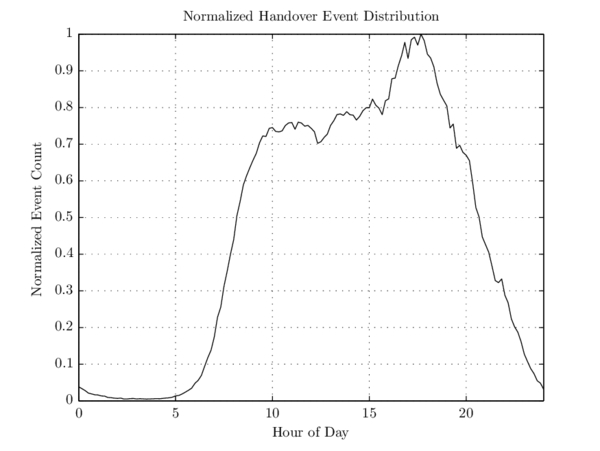
\includegraphics[width=\textwidth]{./images/hauf_event_32_time_mat}
%		\caption{Handover Events}
%		\label{fig:disthandover}
%	\end{subfigure}%
%	~ %add desired spacing between images, e. g. ~, \quad, \qquad etc.
%	%(or a blank line to force the subfigure onto a new line)
%	\begin{subfigure}[b]{0.5\textwidth}
%		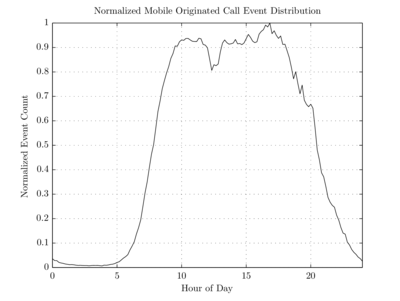
\includegraphics[width=\textwidth]{./images/hauf_event_34_time_mat}
%		\caption{Mobile Originated Calls}
%		\label{fig:distmoc}
%	\end{subfigure}
%	\caption{Normalized Distribution of Handover Events (a) and Mobile Originated Calls on Monday, \nth{22} November 2010}\label{fig:distevents}
%\end{figure}

\subsection{System Overview}
Monitoring units need to be installed in the Core Network of A1 to capture useful events. Fig~\ref{fig:A1Network} illustrates the system architecture used by A1 to capture events. The architecture is almost the same as for a typical GSM system, the only differences are the monitoring units responsible for capturing and forwarding events.
In order to intercept the network, the monitoring units are attached to the main interfaces (A, IuCS, Gb/IuPS, IuPS) of the Core Network. The processing unit is responsible for aggregating events and ensuring anonymity.
\begin{figure}
	\centering
	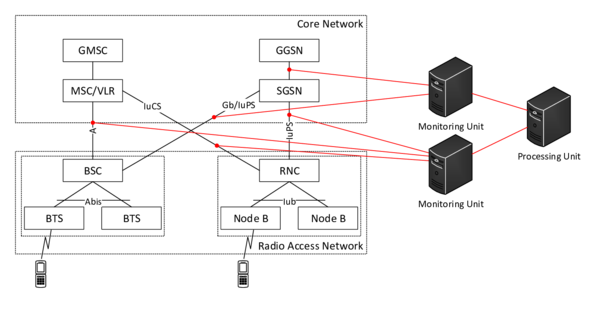
\includegraphics[width=\linewidth]{./images/A1Network}
	\caption{System Architecture of the A1 Monitoring System}
	\label{fig:A1Network}
\end{figure}

\subsubsection{Interfaces}
The monitoring units capture both \emph{Circuit Switched} (CS) and \emph{Packed Switched} (PS) data. Therefore, it intercepts the communication of CS and PS interfaces. The CS interfaces are A and IuCS and they belong to the MSC and enable voice calls and sms. The PS interfaces are the Gb/IuPS and the IuPS. Both are connected to the SGSN and enable subscribers to use packed orientated services (e.g.\ Internet).
%\ subsubsection{Components}
%The monitoring unit is responsible for
\subsection{Data Structure}
\label{sec:dataa1}
Each event captured by the monitoring unit is forwarded to the processing unit for further aggregation. An event is encoded into a binary format and then forwarded to thr consumer. Each event has a fixed length (88 bytes) and its structure is shown in Figure~\ref{fig:a1structure}.
Because not all fields were used by our system, only the ones used are described.

\subsubsection{Anonymous ID}
\label{sec:anonymous}
This 32 bytes field contains a unique anonymous identifier of the mobile terminal. It changes every day at midnight, i.e. a device can be followed for maximum 24 hours time span before the assigned anonymous ID changes.
\subsubsection{Timestamp} The timestamp represents the exact time of occurrence of the event (i.e., the instant when the event has been captured by the monitoring unit).
\subsubsection{Latitude and Longitude}
These two fields represent the position of the BTS in which the event occurred. They are both encoded as decimal numbers representing the WGS84 coordinates in degrees. The decimal number is encoded according to IEEE 754 floating-point double format\cite{IEEE754}.

\subsubsection{Event type}
Every event includes a field (i.e., Event type) that indicates which type of event
has been detected. All possible signaling events are described in Table~\ref{tab:eventtype}.
\subsubsection{Angle}
This field defines the installment of a sector antenna. It is the angle at which the antenna is mounted on the mast. Figure~\ref{fig:antennaangle} illustrates the mounting of a directional antenna on a mast.
%\begin{figure}
%\centering
%\def\svgwidth{200pt}
%\input{images/antennaangle.pdf_tex}
%\caption{Example for a antenna installation}
%\label{fig:antennaangle}
%\end{figure}
\begin{figure}
	\centering
	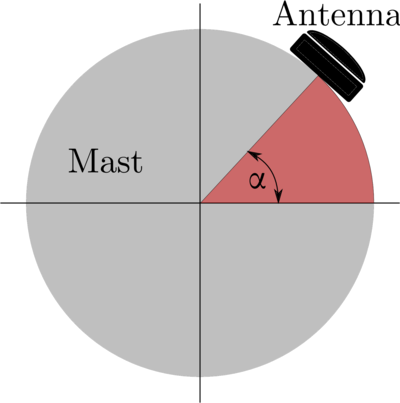
\includegraphics[width=0.4\linewidth]{./images/antennaangle}
	\caption{Example for an antenna installation}
	\label{fig:antennaangle}
\end{figure}

\begin{figure}
	\begin{bytefield}[bitwidth=1.1em]{32}
		\bitheader{0-31} \\
		\wordbox[lrt]{2}{Anonymous ID (32 bytes) } \\
		\skippedwords\\
		\wordbox[lrb]{2}{}\\
		\wordbox{4}{Timestamp (8 bytes)} \\
		\wordbox{4}{Latitude (8 bytes)} \\
		\wordbox{4}{Longitude (8 bytes)} \\
		\wordbox{4}{Radius (8 bytes)} \\
		\bitbox{8}{Source (1byte)}&\bitbox{24}{Reserved (3 bytes)}\\
		\wordbox{2}{Reserved (4 bytes)}\\
		\bitbox{8}{Event (1 byte)}&\bitbox{8}{Reserved (1 byte)} & \bitbox{16}{Reserved (8 bytes)} \\
		\wordbox{4}{Angle (8 bytes)}\\
		\wordbox{2}{Speed (4 bytes)}
	\end{bytefield}
	\caption{Bitstream structure of the A1 Interface}
	\label{fig:a1structure}
\end{figure}
\subsubsection{Encoding example}
The following example illustrates the decoding of the input bit stream.\\
E4A2E4E263A2B54214A2B28E09AE02C36089219123696993EF9E1DF9D8647F18\\
496DC7340006E61B4030747CF7F849A84048143577861E6800000000000005780200\\
00000000000023000000000000000000000000000000
\begin{itemize}
	\item[-] \verb+Anonymous ID+
	      \\Encoded Byte Array = 0xE4A2E4E263A2B54214A2B28E09\-AE02C360\-89219123696993EF9E1DF9D8647F18
	\item[-] \verb|Timestamp:| Wed Jan 14 12:06:28 CET 2009, in microseconds: 1231931188452123
	      \\Encoded Byte Array = 0x496DC7340006E61B

	\item[-] \verb|Latitude:| 16,45503187
	      \\Encoded Byte Array = 0x4030747CF7F849A8
	\item[-] \verb|Longitude:| 48,15788168
	      \\Encoded Byte Array = 0x4048143577861E68
	\item[-] \verb|Radius:| 1400
	      \\Encoded Byte Array = 0x0000000000000578
	\item[-] \verb|Input source:| Metawin
	      \\Encoded Byte Array = 0x02
	\item[-] \verb|Reserved:| 0
	      \\Encoded Byte Array = 0x000000
	\item[-] \verb|Reserved:| 0
	      \\Encoded Byte Array = 0x00000000
	\item[-] \verb|Event type:| Emergency Call
	      \\Encoded Byte Array = 0x23
	\item[-] \verb|Reserved:| 0
	      \\Encoded Byte Array = 0x00
	\item[-] \verb|Reserved:| 0
	      \\Encoded Byte Array = 0x0000
	\item[-] \verb|Angle:| 0
	      \\Encoded Byte Array = 0x0000000000000000
	\item[-] \verb|Speed:| 0
	      \\Encoded Byte Array = 0x0000000
\end{itemize}
\subsection{Events}
\label{subsec:events}
In this subsection, we describe how everyday users activities are visible in the A1 data stream. The events detected by the monitoring units from each terminal depends on the type of terminal. While it is not feasible to cover all events (complete list of events is shown in Tab.~\ref{tab:eventtype}), we only describe the ones --highlighted in the table-- used in our system.

\subsubsection{Calls}
When a terminal establishes a call with another subscriber a Mobile Originated Call event is created. The receiving terminal will create a Mobile Terminated Call event. Whenever a call is ended (e.g.\ one subscriber hangs up)an A Disconnect event is created. However in our research of the data stream, there was no evidence of an A Disconnect event.
\begin{itemize}
	\item MOBILE TERMINATED CALL (0x1D): terminal receives a call
	\item MOBILE ORIGINATED CALL (0x22): terminal originates a call
	\item A DISCONNECT (0x18): The call is closed
\end{itemize}
\subsubsection{Location Area Update}
Devices are most of the time in "idle" mode where they are switched on but are not involved in any voice/data communication. In this state the device must still be reachable by the network. Thus, when a terminal changes to a cell in a different location area, it sends a Location Area Update message to the core network.
This message appears in the data stream as:
\begin{itemize}
	\item LOCATION UPDATE (0x1F), in case of 2G terminal
	\item IUCS LOCATION UPDATE NORMAL (0x15), in case of 3G terminal
\end{itemize}

If a devices do not change its Location Area for a specific time and the PLAU timer expires it sends a keep alive message to the core network.
\begin{itemize}
	\item IUPS RA PERIODIC UPDATE (0x0C) and IUCS LOC UPD PERIODIC
	      (0x17) in case of 3G terminal (for PS and CS domain respectively)
	\item LOCATION UPDATE (0x1F) in case of 2G terminals
\end{itemize}
Figure~\ref{fig:latraversed} illustrates where a location area update (red cell) happens when a subscriber traverses different location areas on its way.
%\begin{figure}
%\centering
%%\def\svgwidth{200pt}
%%\def\svgwidth{400pt}
%\input{images/laupdate.pdf_tex}
%\caption{Cells and location areas traversed by a subscriber}
%\label{fig:latraversed}
%\end{figure}
\begin{figure}
	\centering
	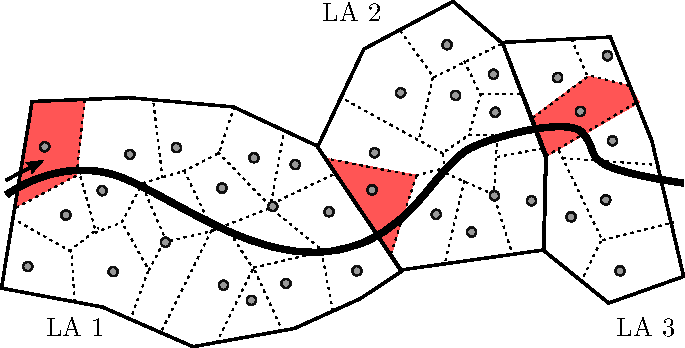
\includegraphics[width=\linewidth]{./images/laupdate.pdf}
	\caption{Cells and location areas traversed by a subscriber}
	\label{fig:latraversed}
\end{figure}

\subsubsection{Handover Cell Update}
When a call is established the terminal is said to be in active "connected" state (see \ref{subsub:connected}).  In this state, the network is informed about each change of
cell, regardless of the LA to which the cell belongs. A limitation is that the A1 data stream is not able to capture cell changes for 3G terminals (these messages do not reach the core network, but terminate in the radio access network,
i.e. they cannot be monitored by the systems).
However cell changes for 2G terminals appear as:
\begin{itemize}
	\item GB CELL CHANGE (0x02), in case of an ongoing data connection,
	\item HANDOVER CELL UPDATE (0x20), in case of an ongoing call.
\end{itemize}


{\small
	\begin{longtable}{|l|p{4cm}|p{8cm}|}
		\hline
		\textbf{HEX} & \textbf{ Event Name}                 & \textbf{Event Description}                                                                                 \\ \hline
		0x01         & GB ATTACH                            & GPRS terminal attaches to the PS                                                                           \\ \hline
		0x02         & GB CELL UPD                          & GPRS terminal changes cell                                                                                 \\ \hline
		0x03         & GB OTHERS                            & GPRS terminal changes cell but message is unclassified                                                     \\ \hline
		0x04         & GB RA UPD                            & GPRS terminal changes RA                                                                                   \\ \hline
		0x05         & IUCS PAGING                          & UMTS terminal is paged in the CS                                                                           \\ \hline
		0x06         & IUPS PAGING                          & UMTS terminal is paged in the PS                                                                           \\ \hline
		0x07         & IU OTHER TLLI                        & UMTS terminal changes cell but message is unclassified                                                     \\ \hline
		0x08         & IU OTHER TMSI                        & UMTS terminal changes cell but message is unclassified                                                     \\ \hline
		0x09         & IUPS ATTACH                          & UMTS terminal attaches to the PS                                                                           \\ \hline
		0x0A         & IUPS DETACH                          & UMTS terminal detaches from the PS                                                                         \\ \hline
		0x0B         & IUPS RA UPD                          & UMTS terminal attached to the PS changes RA                                                                \\ \hline
		0x0C         & IUPS COMB RA/LA UPD                  & UMTS terminal attached to both CS and PS changes LA (and therefore RA)                                     \\ \hline
		0x0D         & IUPS COMB RA/LA UPD WITH IMSI ATTACH & UMTS terminal attaches to the PS and thecurrent RA differs from the one stored in the SIM                  \\ \hline
		0x0E         & IUPS RA PERIODIC UPD                 & UMTS terminal does not change RA for longer than a timer                                                   \\ \hline
		0x0F         & IUCS DETACH                          & UMTS terminal detaches from the CS                                                                         \\ \hline
		0x10         & IUCS SMS ORIGINATED                  & UMTS terminal sends an SMS                                                                                 \\ \hline
		0x11         & IUCS SMS TERMINATED                  & UMTS terminal receives SMS                                                                                 \\ \hline
		0x12         & IUCS SETUP                           & UMTS terminal requests the establishment of a call                                                         \\ \hline
		0x13         & IUCS CONNECT ACK                     & UMTS terminal establishes a call                                                                           \\ \hline
		0x14         & IUCS DISCONNECT                      & UMTS terminal disconnect a call                                                                            \\ \hline
		0x15         & IUCS LOC UPD NORMAL                  & UMTS terminal attached to the CS changes LA                                                                \\ \hline
		0x16         & IUCS LOC UPD PERIODIC                & UMTS terminal does not change LAfor longer than a timer                                                    \\ \hline
		0x17         & IUCS LOC UPD                         & UMTS terminal attaches to the CS and theWITH IMSI ATTACH current LA differs from the one stored in the SIM \\ \hline
		\textbf{0x18}         & \textbf{A DISCONNECT}                         & \textbf{GSM terminal disconnect a call}                                                                             \\ \hline
		0x19         & A OTHER                              & unclassified message on A                                                                                  \\ \hline
		0x1A         & PAGING CS                            & GSM or GPRS terminal is paged in the CS domain                                                             \\ \hline
		0x1B         & DETACH                               & GSM or GPRS terminal detaches from the network                                                             \\ \hline
		0x1C         & SMS                                  & GSM terminal sends or receives an SMS                                                                      \\ \hline
		\textbf{0x1D}         & \textbf{MOBILE TERMINATING CALL}              & \textbf{GSM terminal receives a call}                                                                               \\ \hline
		0x1E         & CM REESTABLISHMENT                   & NA                                                                                                         \\ \hline
		\textbf{0x1F}         & \textbf{LOCATION UPDATE}                      & \textbf{GSM or GPRS terminal changes LA or emits aperiodic RA/LA update or attaches to the network}                 \\ \hline
	\textbf{0x20}          & \textbf{HANDOVER CELL UPDATE}                 & \textbf{GSM terminal in active state changes cell}                                                                 \\ \hline
		0x21         & SUPPLEMENTARY SERVICE                & GSM terminal request a supplementary service                                                               \\ \hline
		\textbf{0x22}         & \textbf{MOBILE ORIGINATED CALL}               & \textbf{GSM terminal originates a call}                                                                             \\ \hline
		0x23         & EMERGENCY CALL                       & GSM terminal establishes an emergency call                                                                 \\ \hline
		0x24         & SETUP                                & GSM terminal request the establishment of a call                                                           \\ \hline
		0x25         & CONNECT ACK                          & GSM terminal establishes a call                                                                            \\ \hline
		0x28         & CLOSURE                              & NA                                                                                                         \\ \hline
		0x29         & GB PS PAGING                         & GPRS terminal is paged in the PS domain                                                                    \\ \hline
		\caption{Description of A1 events}
		\label{tab:eventtype}
	\end{longtable}}
%\begin{table}
%    \begin{tabular}{|lp{2cm}|lp{12cm}|lp{8cm}|}
%    \hline
%    HEX Code & Event Name                            & Event Description                                                                                         \\ \hline
%    0x01     & GB ATTACH                             & GPRS terminal attaches to the PS                                                                          \\ \hline
%    0x02     & GB CELL UPD                           & GPRS terminal changes cell                                                                                \\ \hline
%    0x03     & GB OTHERS                             & GPRS terminal changes cell but message is unclassified                                                    \\ \hline
%    0x04     & GB RA UPD                             & GPRS terminal changes RA                                                                                  \\ \hline
%    0x05     & IUCS PAGING                           & UMTS terminal is paged in the CS                                                                          \\ \hline
%    0x06     & IUPS PAGING                           & UMTS terminal is paged in the PS                                                                          \\ \hline
%    0x07     & IU OTHER TLLI                         & UMTS terminal changes cell but message is unclassified                                                    \\ \hline
%    0x08     & IU OTHER TMSI                         & UMTS terminal changes cell but message is unclassified                                                    \\ \hline
%    0x09     & IUPS ATTACH                           & UMTS terminal attaches to the PS                                                                          \\ \hline
%    0x0A     & IUPS DETACH                           & UMTS terminal detaches from the PS                                                                        \\ \hline
%    0x0B     & IUPS RA UPD                           & UMTS terminal attached to the PS changes RA                                                               \\ \hline
%    0x0C     & IUPS COMB RA/LA UPD                   & UMTS terminal attached to both CS and PS changes LA (and therefore RA)                                    \\ \hline
%    0x0D     & IUPS COMB RA/LA UPD WITH IMSI ATTACH  & UMTS terminal attaches to the PS and thecurrent RA differs from the one stored in the SIM                  \\ \hline
%    0x0E     & IUPS RA PERIODIC UPD                  & UMTS terminal does not change RA for longer than a timer                                                  \\ \hline
%    0x0F     & IUCS DETACH                           & UMTS terminal detaches from the CS                                                                        \\ \hline
%    0x10     & IUCS SMS ORIGINATED                   & UMTS terminal sends an SMS                                                                                \\ \hline
%    0x11     & IUCS SMS TERMINATED                   & UMTS terminal receives SMS                                                                                \\ \hline
%    0x12     & IUCS SETUP                            & UMTS terminal requests the establishment of a call                                                        \\ \hline
%    0x13     & IUCS CONNECT ACK                      & UMTS terminal establishes a call                                                                          \\ \hline
%    0x14     & IUCS DISCONNECT                       & UMTS terminal disconnect a call                                                                           \\ \hline
%    0x15     & IUCS LOC UPD NORMAL                   & UMTS terminal attached to the CS changes LA                                                               \\ \hline
%    0x16     & IUCS LOC UPD PERIODIC                 & UMTS terminal does not change LAfor longer than a timer                                                   \\ \hline
%    0x17     & IUCS LOC UPD                          & UMTS terminal attaches to the CS and theWITH IMSI ATTACH current LA differs from the one stored in the SIM \\ \hline
%    0x18     & A DISCONNECT                          & GSM terminal disconnect a call                                                                            \\ \hline
%    0x19     & A OTHER                               &  unclassified message on A                                                                                \\ \hline
%    0x1A     & PAGING CS                             & GSM or GPRS terminal is paged in the CS domain                                                            \\ \hline
%    0x1B     & DETACH                                & GSM or GPRS terminal detaches from the network                                                            \\ \hline
%    0x1C     & SMS                                   & GSM terminal sends or receives an SMS                                                                     \\ \hline
%    0x1D     & MOBILE TERMINATING CALL               & GSM terminal receives a call                                                                              \\ \hline
%    0x1E     & CM REESTABLISHMENT                    &  NA                                                                                                       \\ \hline
%    0x1F     & LOCATION UPDATE                       &  GSM or GPRS terminal changes LA or emits aperiodic RA/LA update or attaches to the network               \\ \hline
%    0x20     & HANDOVER CELL UPDATE                  &  GSM terminal in active state changes cell                                                                \\ \hline
%    0x21     & SUPPLEMENTARY SERVICE                 &  GSM terminal request a supplementary service                                                             \\ \hline
%    0x22     & MOBILE ORIGINATED CALL                &  GSM terminal originates a call                                                                           \\ \hline
%    0x23     & EMERGENCY CALL                        & GSM terminal establishes an emergency call                                                                \\ \hline
%    0x24     & SETUP                                 & GSM terminal request the establishment of a call                                                          \\ \hline
%    0x25     & CONNECT ACK                           & GSM terminal establishes a call                                                                           \\ \hline
%    0x28     & CLOSURE                               &  NA                                                                                                       \\ \hline
%    0x29     & GB PS PAGING                          &  GPRS terminal is paged in the PS domain                                                                  \\ \hline
%    \end{tabular}
%    \caption {Event table}
%\end{table}


\section{OpenCoverageMap}
OpenCoverageMap was a project and  master thesis done by a colleague of mine at the University of Applied Science Upper Austria. Dieter Schlosser~\cite{Schlosser2012} goal was to create an open network coverage map for mobile networks. Instead of relying on measurements and coverage reports handed out by network operators he was using smartphones that were doing the measurements. This approach, where users a carrying out work, is know as crowd-sourcing~\cite{Surowiecki2004}.
\subsection{Purpose}
In our project, we are using OpenCoverageMap data to evaluate our approaches. In order to measure the network, OpenCoverageMap captures events similar to the events captured by A1.
%The main events are:
%\begin{itemize}
%\item Call establishment
%\item Call termination
%\item Handover update
%\end{itemize}
The OpenCoverageMap application which is installed on the smartphone periodically records the position (using GPS), the phone state as well as the currently connected cell site. Tab.\ \ref{tab:ocmrecord} shows an example of data that was recorded by the OpenCoverageMap application.
\begin{table}[ht]
	\begin{tabular}{|l|l|l|l|l|l|l|}  \hline
		\textbf{Timestamp} & \textbf{Id} & \textbf{Cell-Id} & \textbf{LAC} & \textbf{Latitude} & \textbf{Longitude} & \textbf{State} \\    \hline 1328693325 & 57         & 9884   & 5502 & 48.2443810477206 & 14.2600039950952 & 2 \\  \hline
		1328693326 & 57         & 9884   & 5502 & 48.2443056521896 & 14.2599996518319 & 2\\  \hline
		1328693327 & 57         & 9884   & 5502 & 48.2442309368497 & 14.2600018504158 & 2\\  \hline
		1328693328 & 57         & 9884   & 5502 & 48.2441566900106 & 14.2600058762345 & 2\\  \hline
		1328693329 & 57         & 9884   & 5502 & 48.2440827177131 & 14.2600098594458 & 2\\  \hline
	\end{tabular}
	\caption{Data recorded by OpenCoverageMap for the user 57}
	\label{tab:ocmrecord}
\end{table}
The GPS information allows us to evaluate a route estimated by our system with the actually traveled route (see ~\ref{sec:routevalidation} for more information).
%\subsection{System Architecture}
\subsection{Data Structure}
%\subsection{Conversion}
OpenCoverageMap does not capture events, therefore, our systems needs to covert the OpenCoverageMap data stream to the same format as the A1 data steam. Call establishment and termination events are generated by comparing the timestamps of each record. OpenCoverageMap logs the state of the MS every second. By iterating over the records and comparing the current state with the previous one, it is possible to extract call establishment and termination events. To generate handover events, an iteration over all records is done, each record compares the cell id and lac with the previous one. If both are similar no event is generated. However, if they are different a handover event is generated. After the conversion is done the OpenCoverageMap event stream looks the same as the A1 event stream.
\section{Voronoi Tessellation}
\label{sec:voronoites}
To generate trajectories for each mobile subscriber their coarse location is needed.
For this purpose,we first need an estimation of the coverage area of all cell sites. When a mobile subscriber is connected to a cell site we know that his current position must be withing the coverage area of the cell site. A fast approximation of the coverage area can be done with Voronoi diagrams.
As mentioned before Tettamanti2012 et al.\ \cite{Tettamanti2012} used Voronoi tessellation to estimate the coverage area.

Voronoi diagrams are widely used in computer science, e.g.\ pattern matching, space division, cluster analysis, collision detection, etc.\ as mentioned by Aurenhammer~\cite{Aurenhammer1991}.
\begin{figure}
	\centering
	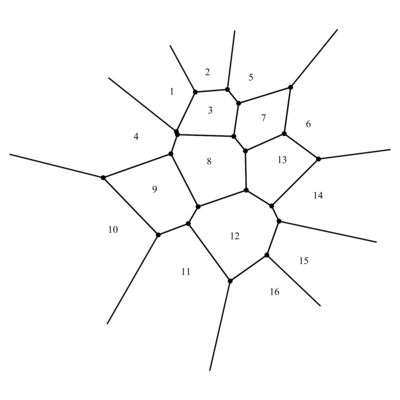
\includegraphics[width=0.7\linewidth]{./images/voronoi2}
	\caption{Voronoi diagram of 16 random points in a 2D space}
	\label{fig:voronoi2}
\end{figure}

\subsection{Point Tessellation}
The following assumptions are based on \emph{Voronoi diagrams--a survey of a fundamental geometric data structure} by Aurenhammer~\cite{Aurenhammer1991} \emph{Computational Geometry: Algorithms and Applications} by Makr de Berg~\cite{Berg2000}.

Let $P=\{p_1,p_2,...,p_n\}$ be a set of $n$ distinct points, in our case the location of each cell site. The Voronoi diagram of $P$ is a subdivision of the plane into $n$ cells. The property that each Voronoi cell must fulfill is that a point $q$ lies in the cell respective to a site $p_i$ only if $dist\left(q,p_i\right) < dist\left(q,p_j\right)$ for each $p_j \in P$ where $i \neq j$. Each cell defines the coverage area for the n-th cell site. Moreover each cell is a (possibly unbounded) open convex polygon. Figure~\ref{fig:voronoi2} illustrates a Voronoi diagram for 16 random points in a two dimensional space. It can be seen that the outer cells are not closed, they shape an open convex polygon. In Section~\ref{sec:boundaries} we show a method to produce closed polygons.
\begin{equation}
	dist(p,q)=\sqrt{\left(p_x-q_x\right)^2+\left(p_y-q_y\right)^2}
\end{equation}
\subsection{Boundaries}
\label{sec:boundaries}
Voronoi diagrams are unbounded which means that the coordinates of vertices can be infinite. Unbounded polygons are undesired in a topology computation. If we would use unbounded polygons for coverage estimation, the area for this cell site would be infinite. A simple approach to eliminate this effect is to clip the Voronoi diagram with a rectangular bounding box. However, this approach is only satisfying if the cell site boundaries shape a rectangle. A better approach is to compute the convex hull over all sites and clip it with the Voronoi diagram.

\subsection{Cell Tower Segmentation}
We mentioned before that a GSM network consists not only of omnidirectional antennas but also of sectored antennas. The coverage area of each sector is defined by the angle at which the antenna is mounted on the tower. If we would only consider the location of each cell sites, sectors with different angles would have the same Voronoi polygon and, therefore, the same coverage area. In order to get a better representation of the coverage area for each sector, we moved the location of each sector based on its angle $\phi$. The definition of the movement can be found in Equation~\ref{eq:move}. The constant factor means a maximum movement of 3 meters in either direction.
\begin{equation}
	\label{eq:move}
	x=x+\frac{cos(\phi)}{50000},y=y+\frac{cos(\phi)}{50000}
\end{equation}
